\bigskip

\item A function is given in Figure 1.10 below.  Which one of the other graphs could be a graph of $f(x+h)$?

% \resizebox{5in}{!}{\includegraphics{SVC.01.03.060.ps}}
\begin{center}
    \begin{tikzpicture}
        \begin{axis}[axis lines=center, xlabel={$x$}, ylabel={$y$}, xmin=-2.5, xmax=2.5,
                ymin=-2.5, ymax=2.5, title={$f(x)$}]
                \addplot[color=blue, very thick,samples=100] {abs(cos(deg(x)))};
            \end{axis}
    \end{tikzpicture}
\end{center}
    
\begin{tikzpicture}
        \begin{axis}[axis lines=center, xlabel={$x$}, ylabel={$y$}, xmin=-2.5, xmax=2.5,
                ymin=-2.5, ymax=2.5, title={Plot (a)}]
                \addplot[color=blue, very thick,samples=100] {abs(cos(deg(x)))-1};
            \end{axis}
        \end{tikzpicture}
    \begin{tikzpicture}
        \begin{axis}[axis lines=center, xlabel={$x$}, ylabel={$y$}, xmin=-2.5, xmax=2.5,
                ymin=-2.5, ymax=2.5, title={Plot (b)}]
                \addplot[color=blue, very thick,samples=100] {abs(cos(deg(x+1)))};
            \end{axis}
        \end{tikzpicture}\\
    \begin{tikzpicture}
        \begin{axis}[axis lines=center, xlabel={$x$}, ylabel={$y$}, xmin=-2.5, xmax=2.5,
                ymin=-2.5, ymax=2.5, title={Plot (c)}]
                \addplot[color=blue, very thick,samples=100] {-0.5*abs(cos(deg(x)))};
            \end{axis}
        \end{tikzpicture}
    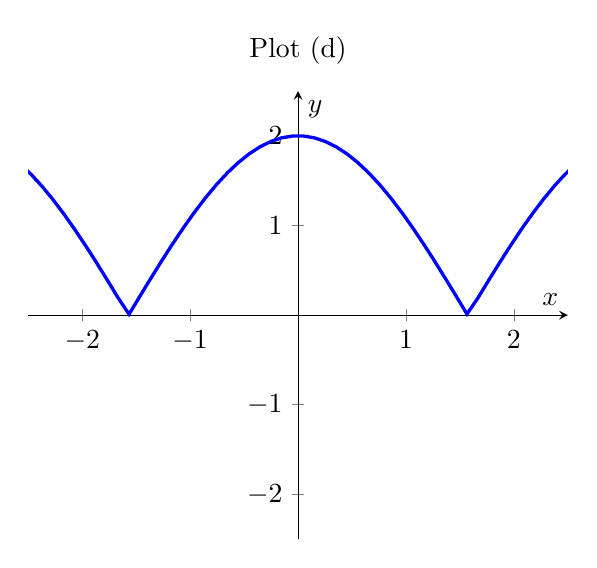
\begin{tikzpicture}
        \begin{axis}[axis lines=center, xlabel={$x$}, ylabel={$y$}, xmin=-2.5, xmax=2.5,
                ymin=-2.5, ymax=2.5, title={Plot (d)}]
                \addplot[color=blue, very thick,samples=100] {2*abs(cos(deg(x)))};
            \end{axis}
        \end{tikzpicture}

% \begin{enumerate}
% \item I
% \item II
% \item III
% \item IV
% \end{enumerate}

% ConcepTests - to accompany Calculus 4th Edition, Hughes-Hallet et al. John Wiley \& Sons.
